\section{Introduction}
Machine Learning (ML), particularly Deep Learning, has significantly advanced the MIR field by enabling automatic feature learning, improving classification and analysis tasks, and facilitating novel applications like music generation and source separation. Adopting musically motivated neural network architectures \cite{musicmotivCNN} blends musical concepts and perceptual approaches and use this knowledge to analyze and understand music in a way that goes beyond traditional music analysis techniques. 

\section{Artificial Neural Networks (ANNs)}
A neural network, formally known as an artificial neural network (ANN), is a computational model inspired by the structure and functionality of biological neural networks. It is a mathematical framework designed to process information and perform tasks like pattern recognition, classification, and regression by mimicking how biological neurons and synapses operate. ANNs comprise interconnected layers of artificial neurons or nodes, each performing a mathematical transformation on the input data to generate an output. The connections between these neurons, often called "weights," are adjusted during learning to optimize the network's performance on a given task.

\subsection{About ANNs}
The concept of neural networks can be traced back to the early 20th century, with the pioneering work of Warren McCulloch and Walter Pitts in 1943. They proposed a mathematical model of a neuron known as the McCulloch-Pitts neuron, which provided a foundation for future research in artificial intelligence. However, Frank Rosenblatt's invention of the perceptron in 1957 marked the beginning of modern neural networks. The perceptron is a single-layer neural network capable of learning linearly separable patterns.

%Single neuron
\begin{SCfigure}[2\sidecaptionrelwidth][h]
	\centering
	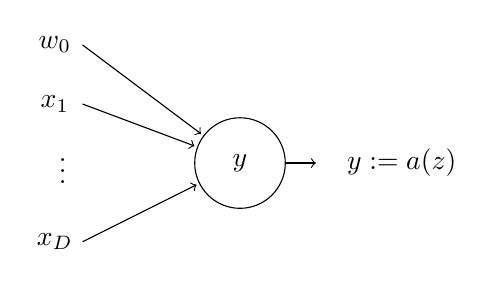
\begin{tikzpicture}[shorten >=1pt,->]
		\tikzstyle{unit}=[draw,shape=circle,minimum size=1.15cm]
 
		\node[unit](p) at (2,1){$y$};
		\node(dots) at (-0.25,1){\vdots};
 
		\draw (0,2.5) node[xshift=-10]{$w_0$} -- (p);
		\draw (0,1.75) node[xshift=-10]{$x_1$} --(p);
		\draw (0,0) node[xshift=-10]{$x_D$} -- (p);
		\draw (p) -- (3,1) node[xshift=30]{$y := a(z)$};
	\end{tikzpicture}
	\caption[Single processing units and its components.]{\small{Single processing unit and its components. The activation function is denoted by $a$ and applied to the actual input $z$ of the unit to form its output $y = a(z)$. $x_1, \ldots, x_D$ represent input from other units within the network; $w_0$ is called bias and represents an external input to the unit. The propagation rule maps all inputs onto the actual input $z$.}}
	\label{fig:processing-unit}
\end{SCfigure}

%NN
\begin{SCfigure}[12][ht]
	\centering
    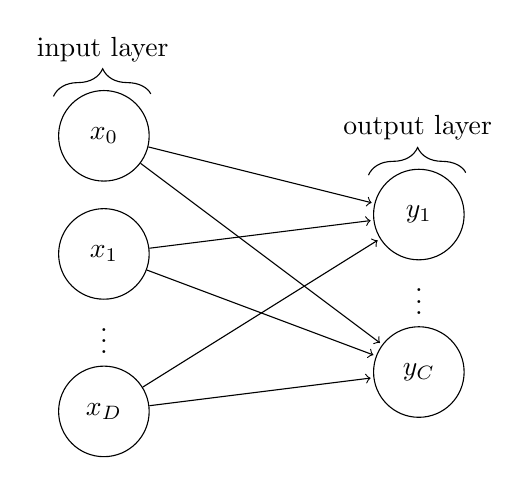
\begin{tikzpicture}[shorten >=1pt]
        \tikzstyle{unit}=[draw,shape=circle,minimum size=1.15cm]
 
        \node[unit](x0) at (0,3.5){$x_0$};
        \node[unit](x1) at (0,2){$x_1$};
        \node(dots) at (0,1){\vdots};
        \node[unit](xd) at (0,0){$x_D$};
 
        \node[unit](y1) at (4,2.5){$y_1$};
        \node(dots) at (4,1.5){\vdots};
        \node[unit](yc) at (4,0.5){$y_C$};
 
        \draw[->] (x0) -- (y1);
        \draw[->] (x0) -- (yc);
 
        \draw[->] (x1) -- (y1);
        \draw[->] (x1) -- (yc);
 
        \draw[->] (xd) -- (y1);
        \draw[->] (xd) -- (yc);
 
        \draw [decorate,decoration={brace,amplitude=10pt},xshift=-4pt,yshift=0pt] (-0.5,4) -- (0.75,4) node [black,midway,yshift=+0.6cm]{input layer};
        \draw [decorate,decoration={brace,amplitude=10pt},xshift=-4pt,yshift=0pt] (3.5,3) -- (4.75,3) node [black,midway,yshift=+0.6cm]{output layer};
    \end{tikzpicture}
    \caption[Network graph of a perceptron with $D$ input units and $C$ output units.]{The perceptron consists of $D$ input units and $C$ output units. All units are labeled according to their output: $y_i = f(z_i)$ in the case of output units; $x_i$ in the case of input units. The input values $x_i$ are propagated to each output unit using the weighted sum propagation rule. The additional input value $x_0 := 1$ is used to include the biases as weights.}
    \label{fig:perceptron}
\end{SCfigure}

In a more technical description, an ANN consists of an input layer, one or more hidden layers, and an output layer. Each neuron in a layer receives input from the previous layer and computes an output value using an activation function. Some standard activation functions include the sigmoid, hyperbolic tangent (tanh), and rectified linear unit (ReLU). The output of the last layer represents the prediction or classification result.

%Activation equation
\begin{figure}
    \centering
    \scalebox{0.8}{
% NEURAL NETWORK activation
% https://www.youtube.com/watch?v=aircAruvnKk&list=PLZHQObOWTQDNU6R1_67000Dx_ZCJB-3pi&index=1
\begin{tikzpicture}[x=2.7cm,y=1.6cm]
\centering
  \message{^^JNeural network activation}
  \def\NI{5} % number of nodes in input layers
  \def\NO{4} % number of nodes in output layers
  \def\yshift{0.4} % shift last node for dots
  
  % INPUT LAYER
  \foreach \i [evaluate={\c=int(\i==\NI); \y=\NI/2-\i-\c*\yshift; \index=(\i<\NI?int(\i):"n");}]
              in {1,...,\NI}{ % loop over nodes
    \node[node in,outer sep=0.6] (NI-\i) at (0,\y) {$a_{\index}^{(0)}$};
  }
  
  % OUTPUT LAYER
  \foreach \i [evaluate={\c=int(\i==\NO); \y=\NO/2-\i-\c*\yshift; \index=(\i<\NO?int(\i):"m");}]
    in {\NO,...,1}{ % loop over nodes
    \ifnum\i=1 % high-lighted node
      \node[node hidden]
        (NO-\i) at (1,\y) {$a_{\index}^{(1)}$};
      \foreach \j [evaluate={\index=(\j<\NI?int(\j):"n");}] in {1,...,\NI}{ % loop over nodes in previous layer
        \draw[connect,white,line width=1.2] (NI-\j) -- (NO-\i);
        \draw[connect] (NI-\j) -- (NO-\i)
          node[pos=0.50] {\contour{white}{$w_{1,\index}$}};
      }
    \else % other light-colored nodes
      \node[node,blue!20!black!80,draw=myblue!20,fill=myblue!5]
        (NO-\i) at (1,\y) {$a_{\index}^{(1)}$};
      \foreach \j in {1,...,\NI}{ % loop over nodes in previous layer
        %\draw[connect,white,line width=1.2] (NI-\j) -- (NO-\i);
        \draw[connect,myblue!20] (NI-\j) -- (NO-\i);
      }
    \fi
  }
  
  % DOTS
  \path (NI-\NI) --++ (0,1+\yshift) node[midway,scale=1.2] {$\vdots$};
  \path (NO-\NO) --++ (0,1+\yshift) node[midway,scale=1.2] {$\vdots$};
  
  % EQUATIONS
  \def\agr#1{{\color{mydarkgreen}a_{#1}^{(0)}}}
  \node[below=17,right=11,mydarkblue,scale=0.95] at (NO-1)
    {$\begin{aligned} %\underset{\text{bias}}{b_1}
       &= \color{mydarkred}\sigma\left( \color{black}
            w_{1,0}\agr{0} + w_{1,1}\agr{1} + \ldots + w_{1,n}\agr{n} + b_1^{(0)}
          \color{mydarkred}\right)\\
       &= \color{mydarkred}\sigma\left( \color{black}
            \sum_{i=1}^{n} w_{1,i}\agr{i} + b_1^{(0)}
           \color{mydarkred}\right)
     \end{aligned}$};
  \node[right,scale=0.9] at (1.3,-1.3)
    {$\begin{aligned}
      {\color{mydarkblue}
      \begin{pmatrix}
        a_{1}^{(1)} \\[0.3em]
        a_{2}^{(1)} \\
        \vdots \\
        a_{m}^{(1)}
      \end{pmatrix}}
      &=
      \color{mydarkred}\sigma\left[ \color{black}
      \begin{pmatrix}
        w_{1,0} & w_{1,1} & \ldots & w_{1,n} \\
        w_{2,0} & w_{2,1} & \ldots & w_{2,n} \\
        \vdots  & \vdots  & \ddots & \vdots  \\
        w_{m,0} & w_{m,1} & \ldots & w_{m,n}
      \end{pmatrix}
      {\color{mydarkgreen}
      \begin{pmatrix}
        a_{1}^{(0)} \\[0.3em]
        a_{2}^{(0)} \\
        \vdots \\
        a_{n}^{(0)}
      \end{pmatrix}}
      +
      \begin{pmatrix}
        b_{1}^{(0)} \\[0.3em]
        b_{2}^{(0)} \\
        \vdots \\
        b_{m}^{(0)}
      \end{pmatrix}
      \color{mydarkred}\right]\\[0.5em]
      {\color{mydarkblue}a^{(1)}}
      &= \color{mydarkred}\sigma\left( \color{black}
           \mathbf{W}^{(0)} {\color{mydarkgreen}a^{(0)}}+\mathbf{b}^{(0)}
         \color{mydarkred}\right)
         %\color{black},\quad \mathbf{W}^{(0)} \in \mathbb{R}^{m\times n}
    \end{aligned}$};

\end{tikzpicture}
}
\caption[Activation function \cite{tikz}.]{\small{The input layer with \textit{n} nodes is denoted as $a_i^{(0)}$ for $i \in \{1, \ldots, n\}$. The output layer with \textit{m} nodes is $a_j^{(1)}$ for $j \in \{1, \ldots, m\}$. Connections between these layers are governed by the weight matrix $\mathbf{W}^{(0)} \in \mathbb{R}^{m\times n}$ and bias vector $\mathbf{b}^{(0)} \in \mathbb{R}^{m}$, with elements $w_{j,i}$ and $b_j^{(0)}$ respectively. The activation function $\sigma$ operates element-wise on the sum of the product of the weight matrix, input vector, and bias vector.}}


    \label{fig:activation_function}

\end{figure}

%Multi-layer_NN
\begin{figure}[ht]
	\centering
	% NEURAL NETWORK with coefficients, shifted
\begin{tikzpicture}[x=2.0cm,y=1.2cm]
  \message{^^JNeural network, shifted}
  \readlist\Nnod{4,5,5,5,3} % array of number of nodes per layer
  \readlist\Nstr{n,m,m,m,k} % array of string number of nodes per layer
  \readlist\Cstr{\strut x,a^{(\prev)},a^{(\prev)},a^{(\prev)},y} % array of coefficient symbol per layer
  \def\yshift{0.5} % shift last node for dots
  
  \message{^^J  Layer}
  \foreachitem \N \in \Nnod{ % loop over layers
    \def\lay{\Ncnt} % alias of index of current layer
    \pgfmathsetmacro\prev{int(\Ncnt-1)} % number of previous layer
    \message{\lay,}
    \foreach \i [evaluate={\c=int(\i==\N); \y=\N/2-\i-\c*\yshift;
                 \index=(\i<\N?int(\i):"\Nstr[\lay]");
                 \x=\lay; \n=\nstyle;}] in {1,...,\N}{ % loop over nodes
      % NODES
      \node[node \n] (N\lay-\i) at (\x,\y) {$\Cstr[\lay]_{\index}$};
      
      % CONNECTIONS
      \ifnum\lay>1 % connect to previous layer
        \foreach \j in {1,...,\Nnod[\prev]}{ % loop over nodes in previous layer
          \draw[connect,white,line width=1.2] (N\prev-\j) -- (N\lay-\i);
          \draw[connect] (N\prev-\j) -- (N\lay-\i);
          %\draw[connect] (N\prev-\j.0) -- (N\lay-\i.180); % connect to left
        }
      \fi % else: nothing to connect first layer
      
    }
    \path (N\lay-\N) --++ (0,1+\yshift) node[midway,scale=1.5] {$\vdots$};
  }
  
  % LABELS
  \node[above=0.8,align=center,mygreen!60!black] at (N1-1.90) {input\\[-0.2em]layer};
  \node[above=0.5,align=center,myblue!60!black] at (N3-1.90) {hidden layers};
  \node[above=1.3,align=center,myred!60!black] at (N\Nnodlen-1.90) {output\\[-0.2em]layer};
  
\end{tikzpicture}
	\caption[Network graph for perceptron.]{\small{Network graph of a perceptron with $D$ input units and $C$ output units. The $l^{\text{th}}$ hidden layer contains $m^{(l)}$ hidden units. Each neuron in a layer receives input from the previous layer and computes an output value using an activation function. The output of the last layer represents the prediction or classification result.
} \cite{tikz}}
	\label{fig: multilayer color perceptron}
\end{figure}

\section{Deep Learning (DL)}

Deep learning is a machine learning subfield that utilizes deep neural networks to learn hierarchical data representations automatically. These networks handle complex, high-dimensional data across domains such as computer vision and natural language processing. Their effectiveness stems from their nonlinear modeling capabilities and scalability with large datasets.

A core algorithm in deep learning is backpropagation which efficiently computes gradients of the loss function concerning the network's parameters. It involves a two-step process: (1) forward pass, where input data propagates through the network to generate predictions, and (2) backward pass, where the error between predictions and ground truth is calculated and propagated back through the network. This process updates the network's parameters using gradient descent, which minimizes the loss function and improves the model's performance.

%Backpropagation
\begin{SCfigure}[2\sidecaptionrelwidth][ht]
	\centering
	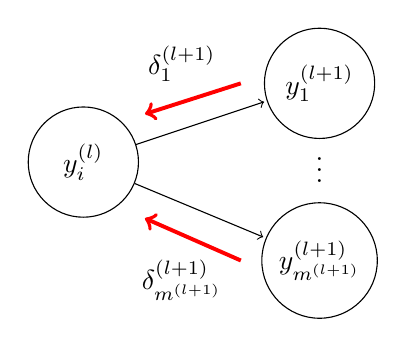
\begin{tikzpicture}[shorten >=1pt]
      		\tikzstyle{unit}=[draw,shape=circle,minimum size =1.4cm]
 
       	\node[unit](i) at (0,1){$y_i^{(l)}$};
        	\node[unit](k1) at (3,2){$y_1^{(l+1)}$};
		\node at (3, 1){$\vdots$};
		\node[unit](km) at (3,-0.25){$y_{m^{(l+1)}}^{(l+1)}$};
		
		\node at (1.25,2.25){$\delta_1^{(l+1)}$};
		\node at (1.25,-0.5){$\delta_{m^{(l+1)}}^{(l+1)}$};
 
        	\draw[->] (i) -- (k1);
		\draw[->] (i) -- (km);
		
		\draw[->,red,line width=0.05cm] (2,-0.25) -- (0.75,0.3);
		\draw[->,red,line width=0.05cm] (2,2) -- (0.75,1.6);
    	\end{tikzpicture}
	\caption[Backpropagation.]{\small{Backpropagation of errors through the network: once evaluated for all output units, the errors $\delta_i^{(L+1)}$ can be propagated backward.}}
	\label{fig:error-backpropagation}
\end{SCfigure}

\subsection{Convolutional Neural Network (CNN)}

A Convolutional Neural Network (CNN) is a deep-learning neural network. The architecture of a CNN is composed of several layers, including:

\begin{itemize}

\item \textbf{Convolutional layers:} These layers apply a convolution operation to the input data. The convolutional layers are designed to effectively learn local patterns and features in the audio data \footnote{For a visual explanation of convolution, see this video: \url{https://youtu.be/KuXjwB4LzSA}}.

A convolution operation involves sliding a small window, called a filter or kernel, over input data to compute the dot product between the kernel and each local region of the data. The result is a new feature map highlighting patterns and essential information.

Given a 2D input data represented as a matrix $I = [i_{ij}]{m \times n}$ and a filter $K = [k{ij}]_{p \times q}$, the convolution operation is defined as:

$$(I * K)_{kl} = \sum_{i=1}^{p} \sum_{j=1}^{q} i_{k+i-1, l+j-1}k_{ij}$$

Here, $k$ ranges from $1$ to $m-p+1$ and $l$ ranges from $1$ to $n-q+1$. The resulting feature map after applying the convolution is denoted by $(I * K)_{kl}$.

The convolution operation slides the kernel $K$ over the input image $I$, performing an element-wise multiplication and sum of the local region centered at pixel $(k,l)$ to compute the value of each element in the output feature map, $(I * K)_{kl}$. This process is repeated for each pixel $(k,l)$, resulting in a new feature map that captures local patterns in the input image.

\begin{center}
\begin{tikzpicture}[
    2d-arr/.style={matrix of nodes, row sep=-\pgflinewidth, column sep=-\pgflinewidth, nodes={draw}}
  ]
  % TikZ code here
  
  \matrix (mtr) [2d-arr] {
  0 & 1 & 1 & |[fill=orange!30]| 1 & |[fill=orange!30]| 0 & |[fill=orange!30]| 0 & 0\\
  0 & 0 & 1 & |[fill=orange!30]| 1 & |[fill=orange!30]| 1 & |[fill=orange!30]| 0 & 0\\
  0 & 0 & 0 & |[fill=orange!30]| 1 & |[fill=orange!30]| 1 & |[fill=orange!30]| 1 & 0\\
  0 & 0 & 0 & 1 & 1 & 0 & 0\\
  0 & 0 & 1 & 1 & 0 & 0 & 0\\
  0 & 1 & 1 & 0 & 0 & 0 & 0\\
  1 & 1 & 0 & 0 & 0 & 0 & 0\\
  };

  \node[below=of mtr-5-4] {$\mathbf I$};

  \node[right=0.2em of mtr] (str) {$*$};

  \matrix (K) [2d-arr, right=0.2em of str, nodes={draw, fill=teal!30}] {
    1 & 0 & 1 \\
    0 & 1 & 0 \\
    1 & 0 & 1 \\
  };
  \node[below=of K-3-2] {$\mathbf K$};

  \node[right=0.2em of K] (eq) {$=$};

  \matrix (ret) [2d-arr, right=0.2em of eq] {
  1 & 4 & 3 & |[fill=blue!80!black!30]| 4 & 1\\
  1 & 2 & 4 & 3 & 3\\
  1 & 2 & 3 & 4 & 1\\
  1 & 3 & 3 & 1 & 1\\
  3 & 3 & 1 & 1 & 0\\
  };
  \node[below=of ret-4-3] {$\mathbf{I * K}$};

  \draw[dashed, teal] (mtr-1-6.north east) -- (K-1-1.north west);
  \draw[dashed, teal] (mtr-3-6.south east) -- (K-3-1.south west);

  \draw[dashed, blue!80!black] (K-1-3.north east) -- (ret-1-4.north west);
  \draw[dashed, blue!80!black] (K-3-3.south east) -- (ret-1-4.south west);

  \foreach \i in {1,2,3} {
      \foreach \j in {4,5,6} {
          \node[font=\tiny, scale=0.6, shift={(-1.2ex,-2ex)}] at (mtr-\i-\j) {$\times \pgfmathparse{int(mod(\i+\j,2))}\pgfmathresult$};
        }
    }
\end{tikzpicture}
\end{center}

%Single CNN
\begin{SCfigure}[2\sidecaptionrelwidth][h]
	\centering
	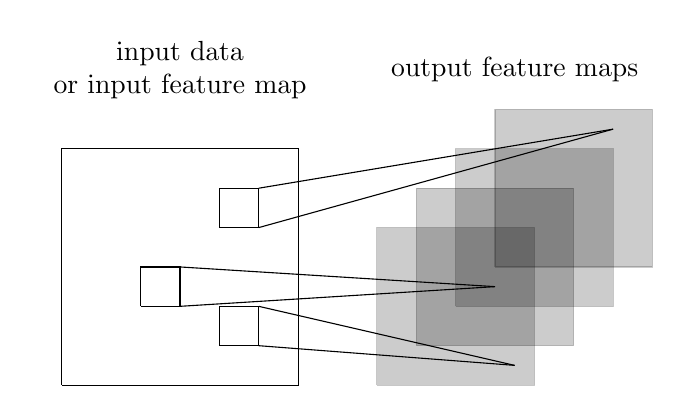
\begin{tikzpicture}
		\node at (1.5,4){\begin{tabular}{c}input data\\or input feature map\end{tabular}};
	
		\draw (0,0) -- (3,0) -- (3,3) -- (0,3) -- (0,0);
		
		\draw (2,2) -- (2.5,2) -- (2.5,2.5) -- (2,2.5) -- (2,2);
		\draw (2,0.5) -- (2.5,0.5) -- (2.5,1) -- (2,1) -- (2,0.5);
		\draw (1,1) -- (1.5,1) -- (1.5,1.5) -- (1,1.5) -- (1,1);
		
		\draw (2.5,2) -- (7,3.25);
		\draw (2.5,2.5) -- (7,3.25);
 
		\draw (2.5,1) -- (5.75,0.25);
		\draw (2.5,0.5) -- (5.75,0.25);
		
		\draw (1.5,1.5) -- (5.5,1.25);
		\draw (1.5,1) -- (5.5,1.25);
		
		\node at (5.75,4){\begin{tabular}{c}output feature maps\end{tabular}};
		
		\draw[fill=black,opacity=0.2,draw=black] (5.5,1.5) -- (7.5,1.5) -- (7.5,3.5) -- (5.5,3.5) -- (5.5,1.5);
		\draw[fill=black,opacity=0.2,draw=black] (5,1) -- (7,1) -- (7,3) -- (5,3) -- (5,1);
		\draw[fill=black,opacity=0.2,draw=black] (4.5,0.5) -- (6.5,0.5) -- (6.5,2.5) -- (4.5,2.5) -- (4.5,0.5);
		\draw[fill=black,opacity=0.2,draw=black] (4,0) -- (6,0) -- (6,2) -- (4,2) -- (4,0);
	\end{tikzpicture}
	\caption[Illustration of a 2D convolutional layer.]{Illustration of a 2D single convolutional layer. If layer $l$ is a convolutional layer, the input data (if $l = 1$) or a feature map of the previous layer is convolved by different filters (or kernels) to yield the output feature maps of layer $l$.}
	\label{fig:convolutional-layer}
\end{SCfigure}

\item \textbf{Pooling layers:} These layers downsample the data, reducing the spatial or temporal dimensions of the input while retaining important information. A joint pooling operation is the max-pooling, which can be defined as follows: given an input matrix $I$ and a pooling window of size $m \times n$, the max-pooling operation selects the maximum value within each non-overlapping $m \times n$ region of the input matrix. This operation effectively reduces the input's dimensions while retaining the essential information in each area.
\vspace*{3mm}

%Single pooling layer
\begin{SCfigure}[2\sidecaptionrelwidth][h]
	\centering
        \scalebox{0.8}{
	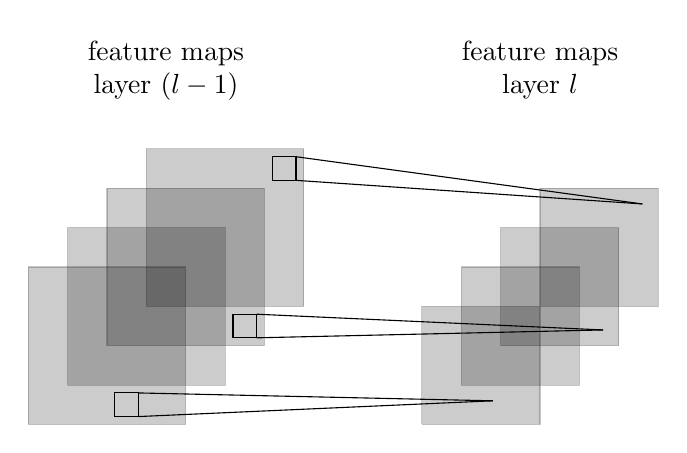
\begin{tikzpicture}
		\node at (1.75,4.5){\begin{tabular}{c}feature maps\\layer $(l-1)$\end{tabular}};
		
		\draw[fill=black,opacity=0.2,draw=black] (1.5,1.5) -- (3.5,1.5) -- (3.5,3.5) -- (1.5,3.5) -- (1.5,1.5);
		\draw[fill=black,opacity=0.2,draw=black] (1,1) -- (3,1) -- (3,3) -- (1,3) -- (1,1);
		\draw[fill=black,opacity=0.2,draw=black] (0.5,0.5) -- (2.5,0.5) -- (2.5,2.5) -- (0.5,2.5) -- (0.5,0.5);
		\draw[fill=black,opacity=0.2,draw=black] (0,0) -- (2,0) -- (2,2) -- (0,2) -- (0,0);
		
		\draw (3.1,3.1) -- (3.4,3.1) -- (3.4,3.4) -- (3.1,3.4) -- (3.1,3.1);
		\draw (2.6,1.1) -- (2.9,1.1) -- (2.9,1.4) -- (2.6,1.4) -- (2.6,1.1);
		\draw (1.1,0.1) -- (1.4,0.1) -- (1.4,0.4) -- (1.1,0.4) -- (1.1,0.1);
		
		\draw (3.4,3.4) -- (7.8,2.8);
		\draw (3.4,3.1) -- (7.8,2.8);
		
		\draw (2.9,1.4) -- (7.3,1.2);
		\draw (2.9,1.1) -- (7.3,1.2);
		
		\draw (1.4,0.4) -- (5.9,0.3);
		\draw (1.4,0.1) -- (5.9,0.3);
		
		\node at (6.5,4.5){\begin{tabular}{c}feature maps\\layer $l$\end{tabular}};
		
		\draw[fill=black,opacity=0.2,draw=black] (6.5,1.5) -- (8,1.5) -- (8,3) -- (6.5,3) -- (6.5,1.5);
		\draw[fill=black,opacity=0.2,draw=black] (6,1) -- (7.5,1) -- (7.5,2.5) -- (6,2.5) -- (6,1);
		\draw[fill=black,opacity=0.2,draw=black] (5.5,0.5) -- (7,0.5) -- (7,2) -- (5.5,2) -- (5.5,0.5);
		\draw[fill=black,opacity=0.2,draw=black] (5,0) -- (6.5,0) -- (6.5,1.5) -- (5,1.5) -- (5,0);
	\end{tikzpicture}
        }
	\caption[Illustration of a pooling and subsampling layer.]{\small{Illustration of a pooling and subsampling layer. If layer $l$ is a pooling and subsampling layer and given $m_1^{(l-1)} = 4$ feature maps of the previous layer, all feature maps are pooled and subsampled individually. Each unit in one of the $m_1^{(l)} = 4$ output feature maps represents the average or the maximum within a fixed window of the corresponding feature map in layer $(l-1)$.}}
	\label{figure: single pooling layer}
\end{SCfigure}

\item \textbf{Fully connected layers:} These layers connect every neuron in one layer to every neuron in another, allowing the network to learn non-linear combinations of the features discovered in the previous layers. Mathematically, a fully connected layer can be represented as $Y = XW + b$, where $X$ is the input matrix, $W$ is the weight matrix, $b$ is the bias vector, and $Y$ is the output matrix. The nonlinearity is introduced through the activation function, which is applied element-wise to the output matrix, such as $Y' = f(Y)$, where $f$ represents the activation function and $Y'$ is the transformed output matrix.
\vspace*{3mm}

\item \textbf{Output layer:} The output layer produces the final predictions of the network.

\end{itemize}

Compared to a traditional neural network, CNNs are more computationally efficient and have less number of parameters to train. This makes them more feasible for large-scale datasets and real-world problems.

On top of that, one of the main advantages of using CNNs for audio analysis is that they can automatically and adaptively learn temporal hierarchies of features from audio data, which traditional audio processing methods may not do effectively. 

%Colour CNN
\begin{figure}[ht]
    \centering
% DEEP CONVOLUTIONAL NEURAL NETWORK
\begin{tikzpicture}[x=1.6cm,y=1.1cm]
  \large
  \message{^^JDeep convolution neural network}
  \readlist\Nnod{5,5,4,3,2,4,4,3} % array of number of nodes per layer
  \def\NC{6} % number of convolutional layers
  \def\nstyle{int(\lay<\Nnodlen?(\lay<\NC?min(2,\lay):3):4)} % map layer number on 1, 2, or 3
  \tikzset{ % node styles, numbered for easy mapping with \nstyle
    node 1/.style={node in},
    node 2/.style={node convol},
    node 3/.style={node hidden},
    node 4/.style={node out},
  }
  
  % TRAPEZIA
  \draw[myorange!40,fill=myorange,fill opacity=0.02,rounded corners=2]
    %(1.6,-2.5) rectangle (4.4,2.5);
    (1.6,-2.7) --++ (0,5.4) --++ (3.8,-1.9) --++ (0,-1.6) -- cycle;
  \draw[myblue!40,fill=myblue,fill opacity=0.02,rounded corners=2]
    (5.6,-2.0) rectangle++ (1.8,4.0);
  \node[right=19,above=1,align=center,myorange!60!black] at (3.1,1.8) {convolutional\\[-0.2em]layers};
  \node[above=1,align=center,myblue!60!black] at (6.5,1.9) {fully-connected\\[-0.2em]hidden layers};
  
  \message{^^J  Layer}
  \foreachitem \N \in \Nnod{ % loop over layers
    \def\lay{\Ncnt} % alias of index of current layer
    \pgfmathsetmacro\prev{int(\Ncnt-1)} % number of previous layer
    %\pgfmathsetmacro\Nprev{\Nnod[\prev]} % array of number of nodes in previous layer
    \message{\lay,}
    \foreach \i [evaluate={\y=\N/2-\i+0.5; \x=\lay; \n=\nstyle;}] in {1,...,\N}{ % loop over nodes
      %\message{^^J  Layer \lay, node \i}
      
      % NODES
      \node[node \n,outer sep=0.6] (N\lay-\i) at (\x,\y) {};
      
      % CONNECTIONS
      \ifnum\lay>1 % connect to previous layer
        \ifnum\lay<\NC % convolutional layers
          \foreach \j [evaluate={\jprev=int(\i-\j); \cconv=int(\Nnod[\prev]>\N); \ctwo=(\cconv&&\j>0);
                       \c=int((\jprev<1||\jprev>\Nnod[\prev]||\ctwo)?0:1);}]
                       in {-1,0,1}{
            \ifnum\c=1
              \ifnum\cconv=0
                \draw[connect,white,line width=1.2] (N\prev-\jprev) -- (N\lay-\i);
              \fi
              \draw[connect] (N\prev-\jprev) -- (N\lay-\i);
            \fi
          }
          
        \else % fully connected layers
          \foreach \j in {1,...,\Nnod[\prev]}{ % loop over nodes in previous layer
            \draw[connect,white,line width=1.2] (N\prev-\j) -- (N\lay-\i);
            \draw[connect] (N\prev-\j) -- (N\lay-\i);
          }
        \fi
      \fi % else: nothing to connect first layer
      
    }
  }
  
  % LABELS
  \node[above=0.5,align=center,mygreen!60!black] at (N1-1.90) {input\\[-0.2em]layer};
  \node[above=1.5,align=center,myred!60!black] at (N\Nnodlen-1.90) {output\\[-0.2em]layer};
  
\end{tikzpicture}
    \caption{High-level illustration of a CNN}
    \label{fig: CNN colour diagram}
\end{figure}

\newpage


